\chapter{Background}
The system is split into three different parts, the website, raspberry pi and the cloud(Azure), these are also split in their respective parts with website containing the webserver(node) and the site(React), the Cloud; 
\begin{itemize}
  \item Azure sql server
  \item Azure sql database
\end{itemize}



\section{Website}
A website is often confused with a webpage or a web server. From mozillaWebDoc, A website is a collection of web pages which are grouped together in various ways. A web server hosts websites and their supporting files are available on the that computer. 
How do they talk to each other?
A website talks to the webserver using an API, which is a connection between to computer programs. It could be referred also as the specification or as the implementation, the specification has to do with a document that demonstrates how to use or create a connection. Examples of API specifications used in this project are; tedious for the database connection to azure, express as a middleware. 

MVC architecture.

middleware for NodeJS.
\subsection{Node}


\subsection{React}




\newacronym{API}{$API$}{Application Programming Interface}
\glsadd{API}
reason for a website is to allow the Admin or Lecturer access this system from anywhere so that he can start tracking attendance from anywhere.

\section{Raspberry-pi}
A portable computer with 40 GPIO pins, 
GPIO is an uncommitted digital pin on an electronic circuit board which may be used as input or output or both, and can be configured by the user at runtime[6]. This GPIO allows to interface with different modules. A module here is a small unit that can be integrated into a larger system but also maintained separately with no effect on the system. It is of a "plug-in" functionality.
To connect to azure from the raspberry pi, "pyodbc" driver is used. The driver files are installed on the raspberry-pi
LED  

\newacronym{GPIO}{$GPIO$}{General Purpose Input Output}
\glsadd{GPIO}

\subsection{RFID - RC522}
The RFID card interfaces with the raspberry-pi with SPI communication, it is a synchronous serial communication that encourages communication over a short distance, it is mainly used in embedded systems. Serial communication has to do with sending one bit at a time sequentially and synchronous means that this communication is synchronized by a clock signal which is used orchestrate the actions of the digital circuit i.e to determine when it is time to read the next bit/value. SPI devices communicate in a full duplex mode with a master-slave principle normally with a single master. full duplex means that data is transmitted back and forth simultaneously in this communication channel.

% \vspace{1cm}
\begin{figure}[h]
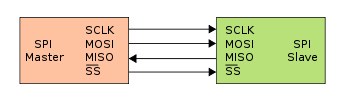
\includegraphics{Background/images/350px-SPI_single_slave.svg.png.png}
\end{figure}
\newacronym{SPI}{$SPI$}{Serial Peripheral Interface}
\glsadd{SPI}

SPI has four main logic signals: 
\begin{itemize}
  \item SCLK: Serial clock, which is gotten from the master
  \item MOSI: Master Out Slave In, is data from the master
  \item MISO: Master In Slave Out, is data from the slave
  \item CS/SS: Chip/Slave Select, an output from the master to notify data is being transmitted.
\end{itemize}

For RC522, there are other logical signals such as;
\begin{itemize}
  \item SDA: 1\textsuperscript{2}C-bus serial data line input/output 
  \item SCK: SPI serial clock input which is same as SCLK
  \item GND: for ground connection
  \item 3.3v: which powers the RC522 module
\end{itemize}


RFID uses electromagnetic fields to detect 

RFID tags are classified by their frequencies, the four primary frequency ranges are:
\begin{itemize}
  \item Low frequency (LF): they are include frequencies from 30 to 300KHz
  \item High frequency (HF)
  \item Ultra high frequency (UHF)
  \item Microwave frequency (microwave)
\end{itemize}

13.56GHz frequency 

The rfid has a uniqueID


\subsection{Fingerprint - R3}
The Fingerprint interfaces with the Raspberry pi with UART communication, it is a devices that supports asynchronous serial communication, which is a form of serial communication that doesn't require a clock signal and is not constantly synchronized. 

Raspberry pi supports asynchronous communication but with a lot of fingerprints having distinct voltages, I used a USB to UART Converter which supports both 3.3v and 5v although the R3 is 3.3v. The TX pin goes to RX pin and vice versa in the connection between the converter and fingerprint module.




\newacronym{UART}{$UART$}{Universal Asynchronous Receiver-Transmitter}
\glsadd{UART}



\section{Cloud - Azure}
AzureSQL server hosts the SQL database and handles connection to other devices, programs or services. Relational Database?



